% !Mode:: "TeX:UTF-8"
% VL 13, gebaut aus part-architekturen-anwendungen/22-gans.md und dem Induktionsteil
% von part-lernen/09-backpropagation.md (Wiederholung vor der Klausur).
% (Dialogmuster und Zeiten: transcripts/vl12-gans-2025/notiz.md).
% !Mode:: "TeX:UTF-8"
\newcommand{\thepage}{} % to silence a hyperref warning about pdfpagelabels
\RequirePackage[]{silence}
\WarningsOff[hyperref]
\PassOptionsToPackage{log-declarations=false}{xparse}
%\RequirePackage[l2tabu, orthodox]{nag}
\RequirePackage{luatex85} % to make \pdf...= commands work with LuaTeX
\documentclass[aspectratio=169,t]{beamer}
\usepackage{ifthen}
\usepackage[T1]{fontenc}
\usepackage{iftex}
\ifLuaTeX
 \usepackage{fontspec}
 \setmainfont[Ligatures=TeX]{Source Sans Pro}
\else
 \usepackage[utf8]{inputenc}
\fi
\usepackage{german}
\usepackage{newunicodechar}
\newunicodechar{€}{\texteuro}
\newunicodechar{ß}{\ss}
\renewcommand{\SS}{\iffontchar\font"1E9E \symbol{"1E9E}\else SS\fi}
\usepackage{ellipsis}
\usepackage{microtype}
\usepackage{listings}
\usepackage{sourcecodepro}
\lstset{language=Python, basicstyle=\ttfamily}
\usepackage{amsfonts}
\usepackage{amssymb}
\usepackage{amsthm}
\usepackage{fancyhdr}
\usepackage{graphicx}

\newtheorem{proposition}[theorem]{Proposition}

\DeclareMathOperator*{\argmax}{argmax}
\DeclareMathOperator{\supp}{supp}
\newcommand{\E}{\ensuremath{\mathbb{E}}}
\newcommand{\V}{\ensuremath{\mathbb{V}}}

\setbeamercolor{emph}{fg=purple}
\renewcommand<>{\emph}[1]{%
  {\usebeamercolor[fg]{emph}\only#2{\itshape}#1}%
}



\hypersetup{draft=false,colorlinks=false,pdfpagemode=UseOutlines,plainpages=false,
            breaklinks=true,bookmarksnumbered=true,pdfborder=0 0 0,
            pdftitle={Einführung in Deep Learning WiSe 2026/27 HHU},
            pdfauthor={Konrad Voelkel},
            pdfsubject={data science}}

%\documentclass[aspectratio=169,t]{beamer}
\usetheme{hhubeamer} % put the hhu-beamer-theme in /usr/share/texmf/tex/latex/beamer/themes/

% -------------------- Code listings config --------------------
% Define custom colors for syntax highlighting
\definecolor{codegreen}{rgb}{0,0.6,0}
\definecolor{codegray}{rgb}{0.5,0.5,0.5}
\definecolor{codepurple}{rgb}{0.58,0,0.82}
\definecolor{backcolour}{rgb}{0.96,0.96,0.94} % Very light gray/beige
% Configure the listings package
\lstset{
    language=Python,
    backgroundcolor=\color{backcolour},   
    commentstyle=\color{codegreen}\itshape,
    keywordstyle=\color{blue}\bfseries,
    numberstyle=\tiny\color{codegray},
    stringstyle=\color{codepurple},
    basicstyle=\ttfamily\footnotesize, % Use a monospaced font
    breakatwhitespace=false,         
    breaklines=true,      
             % Enable automatic line breaking
    captionpos=b,                      % Caption at the bottom
    keepspaces=true,                 
    numbers=left,                      % Line numbers on the left
    numbersep=10pt,                    % Distance of line numbers from the code
    showspaces=false,                
    showstringspaces=false,            % Don't show weird underscores in strings
    showtabs=false,                  
    tabsize=4,
    frame=single,                      % Add a subtle border around the code
    rulecolor=\color{black!20},        % Border color
  }

\event[]{}
\author[Wintersemester 2026/27]{Dr. Konrad Völkel, Wintersemester 2026/27}

%\title{Data Science, VL 1}
%\date{16.04.2026}


%%% Local Variables:
%%% mode: latex
%%% TeX-master: t
%%% End:


% Fassung mit Dozentennotizen (zweiter Schirm): die nächste Zeile einkommentieren.
% \setbeameroption{show notes on second screen=right}

\graphicspath{{../images/}}

\title[GANs (VL 13)]{GANs -- und Backpropagation als Induktion\\\large Einführung in Deep Learning, VL 13}
\date{20.01.2027}

\begin{document}

\begin{frame}
  \titlepage

  \note{\textbf{Ablauf, 90 Minuten} (2025 hat die GAN-Sitzung 60 Min. gebraucht und
    bewusst früher geschlossen -- die frei werdende Zeit geht dieses Jahr in die
    Backprop-Wiederholung, die klausurrelevant ist):\\[2pt]
    \begin{tabular}{@{}rll@{}}
      0--4   & Folie 2       & Probeklausur, Ablauf bis zur Klausur\\
      4--12  & Folien 3--4   & 2014: zwei Netze gegeneinander\\
      12--24 & Folien 5--6   & Generator, Diskriminator, Minimax\\
      24--36 & Folien 7--8   & Training abwechselnd, Gleichgewicht\\
      36--46 & Folie 9       & \textbf{GAN Lab live}\\
      46--56 & Folien 10--11 & Conditional GANs, Mode Collapse\\
      56--64 & Folie 12      & Wasserstein-GAN, kurz\\
      64--86 & Folien 13--16 & \textbf{Backpropagation als Induktion (Wiederholung)}\\
      86--90 & Folie 17      & Probeklausur, Fragestunde\\
    \end{tabular}\\[4pt]
    Beim GAN Lab die Regel aus 2025 beachten: \emph{früh aufhören}. Nach etwa zehn
    Minuten kippt es in Mode Collapse, und das ist genau der Moment zum Weitergehen.}
\end{frame}

\begin{frame}
  \frametitle{Wo wir stehen}

  \begin{center}
    \Large
    Heute: das letzte neue Modell des Semesters.\\[16pt]
    Und danach: Backpropagation noch einmal -- klausurrelevant.
  \end{center}

  \note{Die Probeklausur kommt heute raus, Abgabe nächste Woche. Das letzte
    reguläre Blatt ist abgegeben.
    Die Wiederholung in der zweiten Hälfte ist ausdrücklich Klausurvorbereitung --
    Aufgabentyp 4 ist die Backprop-Rechnung.}
\end{frame}

\begin{frame}
  \frametitle{2014: zwei Netze gegeneinander}

  \begin{center}
    \Large
    Goodfellow et al., \emph{Generative Adversarial Nets}\\[16pt]
    \normalsize kein Markov-Chain-Sampling,\\ keine Variationsrechnung --\\
    nur zwei Netze und Backpropagation.
  \end{center}

  \note{Yann LeCun 2016 auf Quora: die wichtigste Idee der letzten Jahre im Deep Learning.
    Der Kontrast zum VAE ist wichtig: Dort haben wir mit KL-Termen und
    Reparametrisierungstrick gearbeitet. Hier braucht es nichts davon.}
\end{frame}

\begin{frame}
  \frametitle{Der Aufbau}

  \begin{center}
    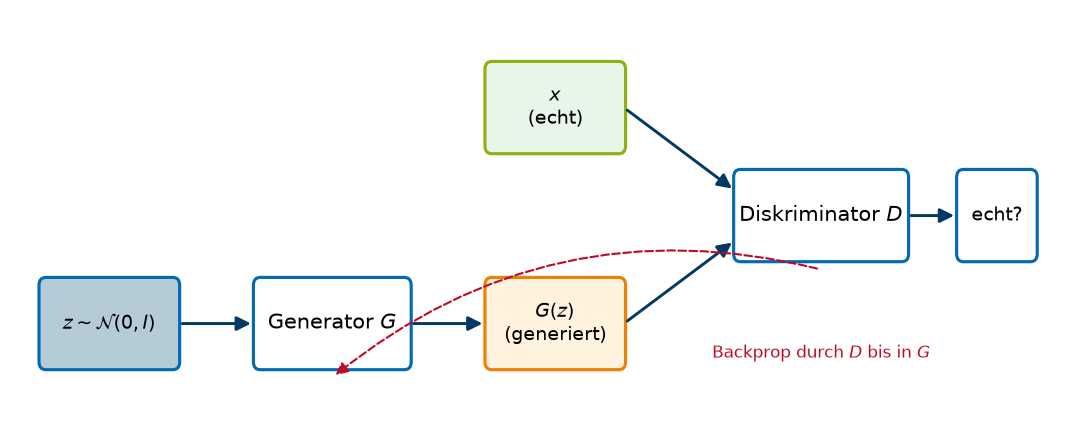
\includegraphics[width=0.66\textwidth]{vl12-gan-schema.png}
  \end{center}

  \note{Der \emph{Generator} bekommt Rauschen $z \sim \mathcal{N}(0,I)$ und macht daraus
    ein Bild. Der \emph{Diskriminator} bekommt ein Bild -- echt oder generiert -- und
    soll sagen, was es ist.
    \textbf{Die Pointe, die man betonen sollte:} Der Generator sieht \emph{nie} echte
    Daten. Er sieht nur den Gradienten, der durch den Diskriminator zurückfließt.}
\end{frame}

\begin{frame}
  \frametitle{Beides kennen wir schon}

  \begin{center}
    \Large
    Generator $=$ Decoder (VL 8)\\[14pt]
    Diskriminator $=$ Klassifikator (VL 4)
  \end{center}

  \note{Das ist die Take-Home-Message der Sitzung: Ein GAN ist nichts Neues, sondern zwei
    Netze, die wir schon kennen, mit Backpropagation gegeneinander trainiert.
    Der Generator kann sogar der Decoder eines vortrainierten Autoencoders sein -- dann
    hat man schon einen brauchbaren latenten Raum.}
\end{frame}

\begin{frame}
  \frametitle{Das Minimax-Spiel}

  \begin{center}
    \Large
    $\min_G \max_D\; \mathbb{E}_{x}\bigl[\log D(x)\bigr]
      + \mathbb{E}_{z}\bigl[\log(1 - D(G(z)))\bigr]$
  \end{center}

  \bigskip
  \begin{center}
    \normalsize Das ist die BCE des Diskriminators.
  \end{center}

  \note{\textbf{Diese Formel gehört auf die Folie} -- 2025 fehlte sie und wurde vermisst.
    Label 1 für echt, 0 für generiert. $D$ will maximieren (gut klassifizieren), $G$ will
    minimieren ($D$ täuschen).
    Also: dieselbe binäre Kreuzentropie wie in VL 5, nur mit zwei Parteien, die in
    entgegengesetzte Richtungen daran ziehen.}
\end{frame}

\begin{frame}
  \frametitle{Training: abwechselnd}

  \begin{center}
    \Large
    \textbf{D-Schritt}: ein Batch echt (Label 1), ein Batch generiert (Label 0)\\[14pt]
    \textbf{G-Schritt}: Rauschen rein, Penalty dafür,\\ dass $D$ „generiert“ sagt
  \end{center}

  \note{Der Diskriminator wird für falsch positive \emph{und} falsch negative bestraft.
    Der Generator kann vorher als Decoder eines Autoencoders vortrainiert werden, damit
    er die Verteilung grob kennt -- dann ist das GAN-Training Finetuning.
    Frage in den Raum: Was passiert, wenn einer von beiden zu gut wird?}
\end{frame}

\begin{frame}
  \frametitle{Das Gleichgewicht}

  \begin{center}
    \Huge $D \equiv \tfrac12$
  \end{center}

  \bigskip
  \begin{center}
    \normalsize Wenn $G$ die Datenverteilung trifft, kann $D$ nur noch raten.
  \end{center}

  \note{Das ist das Ziel -- und eine hübsche Umkehrung der üblichen Logik: Ein
    Klassifikator, der nur noch rät, ist normalerweise ein schlechtes Ergebnis. Hier ist
    er der Beweis, dass der Generator gut ist.
    Verallgemeinerung, die 2025 gut ankam: Jeden Klassifikator, der echt von generiert
    unterscheidet, kann man als Trainingssignal nehmen und genau diesen Unterschied
    weglernen.}
\end{frame}

\begin{frame}
  \frametitle{Ausprobieren: GAN Lab}

  \begin{center}
    \Large poloclub.github.io/ganlab
  \end{center}

  \bigskip
  \begin{center}
    \normalsize Generator-Verteilung, Gradientenfeld, Loss-Kurven -- live.
  \end{center}

  \note{\textbf{Browser-Block, etwa zehn Minuten -- und dann aufhören.} Das ist die Regel
    aus 2025: Bei der Ring- oder Gauß-Wolke wandert die Generator-Verteilung erst schön
    hin, danach kippt es meist in Mode Collapse.
    Genau diesen Moment kann man zeigen und dann zur nächsten Folie gehen: Man hat gerade
    live gesehen, was das Problem ist.}
\end{frame}

\begin{frame}
  \frametitle{Conditional GANs}

  \begin{center}
    \Large
    $G(z, y)$ und $D(x, y)$
  \end{center}

  \bigskip
  \begin{center}
    \normalsize Jetzt kann man sagen, \emph{welche} Ziffer gezeichnet werden soll.
  \end{center}

  \note{Zusatzinformation für beide -- meistens das Klassenlabel.
    Das ist der Schritt von „irgendein Gesicht“ zu „ein Gesicht mit Brille“, und der
    Vorläufer von Text-zu-Bild.}
\end{frame}

\begin{frame}
  \frametitle{Zwei Probleme}

  \begin{center}
    \Large
    \textbf{Mode Collapse}: immer dasselbe Bild\\[16pt]
    \textbf{Vanishing Gradients}: $D$ wird zu schnell zu gut
  \end{center}

  \note{Mode Collapse: Die Verteilung kollabiert auf wenige Punkte, die $D$ gerade nicht
    erkennt. Genau das hat man im GAN Lab gesehen.
    Vanishing Gradients: Ist $D(G(z)) \approx 0$ überall, dann ist $\log(1 - D(G(z)))$
    flach und der Generator lernt nichts mehr -- dasselbe Phänomen wie bei den sterbenden
    Neuronen in VL 7.}
\end{frame}

\begin{frame}
  \frametitle{Wasserstein-GAN}

  \begin{center}
    \Large
    Statt „echt oder generiert?“:\\[10pt]
    \emph{wie weit} sind die beiden Verteilungen auseinander?
  \end{center}

  \note{Die Wasserstein-Distanz (earth mover's distance) gibt auch dann noch einen
    brauchbaren Gradienten, wenn der Diskriminator sicher ist -- deshalb hilft sie gegen
    beide Probleme.
    Der Kritiker gibt eine reelle Zahl aus, keine Wahrscheinlichkeit; der Wertebereich ist
    nicht $[0,1]$. Die Dualität steht als Vertiefung im Skript und ist nicht
    klausurrelevant.}
\end{frame}

% ------------------------------------------------------------------ Backprop-Wiederholung
\begin{frame}
  \frametitle{Wiederholung: Backpropagation}

  \begin{center}
    \Large
    Warum funktioniert das eigentlich \emph{immer}?
  \end{center}

  \note{Übergang ansagen: Der Rest der Sitzung ist Wiederholung und Klausurvorbereitung.
    In VL 6 haben wir es an einem Beispiel gerechnet. Jetzt die Formulierung, mit der man
    \emph{jede} Architektur erschlägt -- als Induktion.}
\end{frame}

\begin{frame}
  \frametitle{Forward Pass}

  \begin{center}
    \Large
    Für jede Operation speichern:\\[12pt]
    das Zwischenergebnis,\\
    die Ableitung der Operation,\\
    worauf sie zurückgreift.
  \end{center}

  \note{Das ist der Aufbau des DAG. Mehr passiert im Vorwärtsdurchlauf nicht -- und genau
    das haben wir in VL 12 im Code gesehen: \texttt{grad\_fn} und saved tensors.}
\end{frame}

\begin{frame}
  \frametitle{Der Induktionsschritt}

  \begin{center}
    \Large
    $\dfrac{d}{dw_Y} Z\bigl(Y(x; w_Y); w_Z\bigr)
      = \dfrac{dZ}{dy} \cdot \dfrac{dY}{dw_Y}$
  \end{center}

  \bigskip
  \begin{center}
    \normalsize Bekannt: $dY/dw_Y$ (Induktionsvoraussetzung) und $dZ/dy$ (neue Operation).
  \end{center}

  \note{$Y$ sind „die bisherigen Rechenoperationen“, $Z$ ist „die nächste“. Mehr braucht
    die Kettenregel nicht.
    Mit vollständiger Induktion folgt: \emph{Ein} Durchlauf durch den DAG liefert alle
    Ableitungen -- insbesondere den Loss nach allen Gewichten.
    In diese Rechnung fließt null Kreativität. Das ist der Grund, warum es ein Computer
    kann.}
\end{frame}

\begin{frame}
  \frametitle{Was in der Klausur drankommt}

  \begin{center}
    \Large
    Ein kleines Netz, kleine Zahlen,\\
    Forward, Backward, ein Update.
  \end{center}

  \bigskip
  \begin{center}
    \normalsize Immer dazuschreiben, \emph{wonach} abgeleitet wird.
  \end{center}

  \note{Aufgabentyp 4 aus dem Aufgabenschatz. Das Rechenbeispiel vom Übungsblatt ist die
    Blaupause.
    Der häufigste Fehler bleibt derselbe: nicht dazuschreiben, wonach abgeleitet wird --
    das kostet jedes Jahr Punkte.
    Wenn Zeit bleibt: das Faltungsbeispiel aus VL 12 als zweite Übung rechnen, da kommt
    das Summieren geteilter Gewichte dazu.}
\end{frame}

\begin{frame}
  \frametitle{Probeklausur}

  \begin{itemize}\setlength{\itemsep}{8pt}
  \item Ab heute in ILIAS, Abgabe nächsten Mittwoch
  \item Besprechung in der Übung nächste Woche
  \end{itemize}

  \bigskip
  \begin{center}
    Nächste Woche: latente Räume und Anwendungsbeispiele.
  \end{center}

  \note{Die Probeklausur ersetzt das letzte Übungsblatt. Ernst nehmen: Sie ist im Format der
    echten Klausur, sechs Aufgaben, 90 Minuten.
    Wer mag, schreibt sie unter Prüfungsbedingungen -- das ist die beste Vorbereitung.}
\end{frame}

\end{document}

%%% Local Variables:
%%% mode: latex
%%% TeX-master: t
%%% End:
